\documentclass[../main.tex]{subfile}

\begin{document}

\section{Le rêve insinué}

La base même d'un rêve est les sensations qu'il produit pour le sujet. Ces
sensations sont au-délà des simples informations sur le monde extérieur
auquelles nous sommes habitués. Elles présentes certaines caractéristiques qui
sont intéressantes à reproduire pour imiter cet effet.

Généralement, un rêve est accompagné d'un état inconscient (sauf dans le cas
d'un \emph{rêve lucide}). C'est le premier outil à disposition du réalisateur :
si le spectateur ne sait pas qu'il observe un rêve, l'effet est accru au moment
où il s'en rend compte.

Cependant, cette idée est bien plus difficile à réaliser qu'il n'y paraît. Un
spectateur n'a a sa disposition que \emph{la vue} et \emph{l'ouïe} comme canaux
de communication avec l'univers du film regardé. Pourtant, au sein d'un rêve,
le sujet perçoit une grande variété de sensations différentes. C'est donc un
problème majeur pour la reproduction d'un rêve dans une \oe{}uvre
cinématographique.

\subsection{Aspect visuel}

Le cinéma est avant tout un \textbf{art photographique}, et à l'origine n'était
qu'une projection d'images sensées reproduire une histoire pour le spectateur.

La représentation visuelle d'un rêve est cruciale car c'est le moyen de
dialogue privilégié entre le réalisateur et le spectateur.

\subsubsection{Lenteur des images}

Pour simuler l'état d'inconscience accompagnant le rêve, le spectateur est
souvent entraîné dans une hypnose partielle, notamment à travers une lenteur
exagérée des images.

On peut voir par exemple dans \emph{Lost Highway (1997)} (figure
\ref{fig:images_lynch}), des longs plans centrés sur la route, qui semble se
dérouler à l'infini devant nous.

Pour le spectateur assis confortablement depuis un certain temps dans une salle
sombre, souvent avec une musique douce et pesante, l'effet est net.

\begin{figure}[htpb]
    \centering
    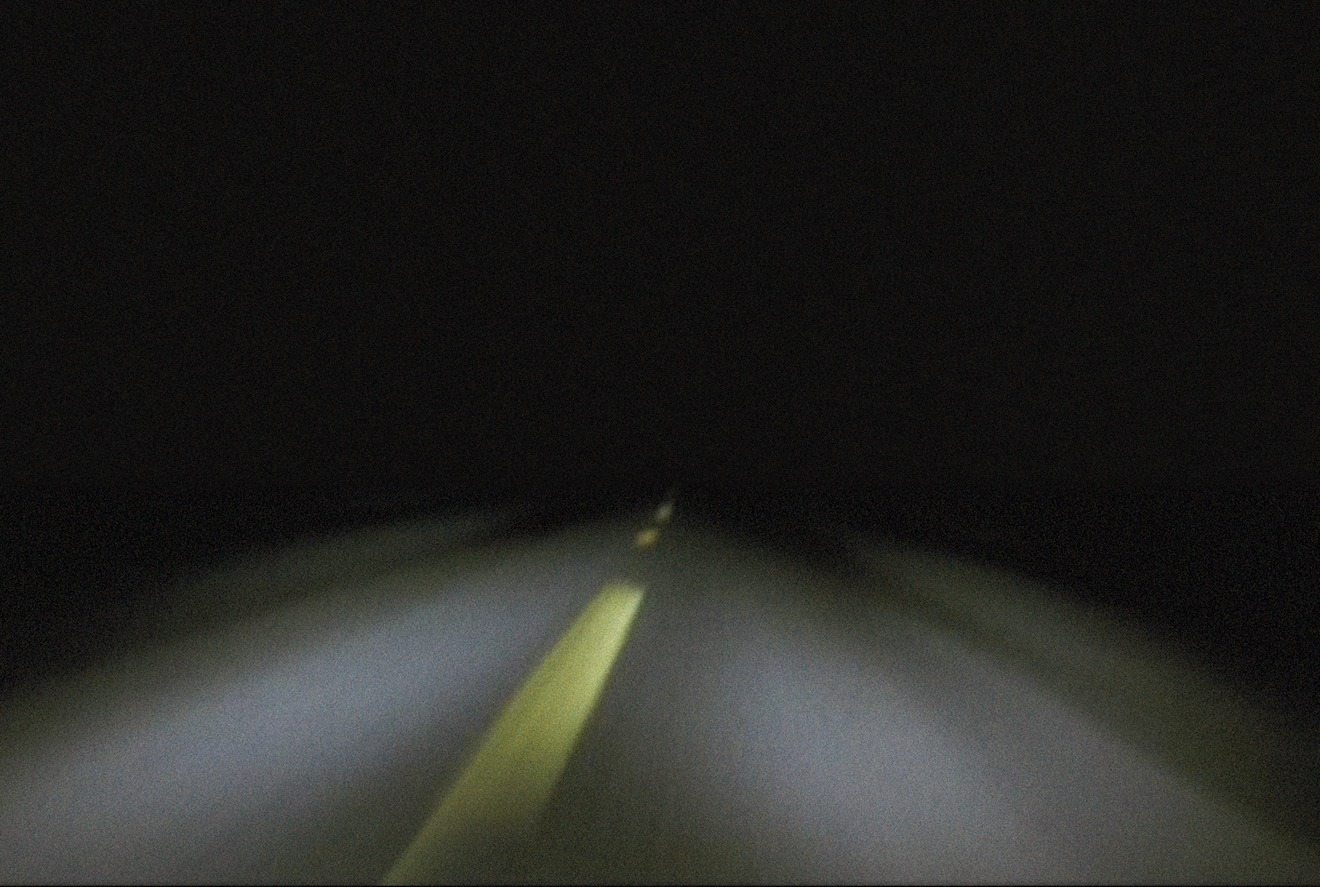
\includegraphics[width=\linewidth]{images/lynch}
    \caption{Extrait de Lost Highway (1997), un film de David Lynch}
    \label{fig:images_lynch}
\end{figure}

\subsubsection{Abondance de couleurs}

Une technique de représentation est l'utilisation excessive de
\textbf{contrastes de couleurs}. Cette méthode a l'avantage de captiver le
regard du spectateur sans pour autant trop en dire sur l'environnement.

En effet, le cinéma étant un art photographique, le spectateur peut confondre
la vision imposée par le réalisateur avec celle perçue par le(s) personnage(s)
dans le film.

\begin{figure}[htpb]
    \centering
    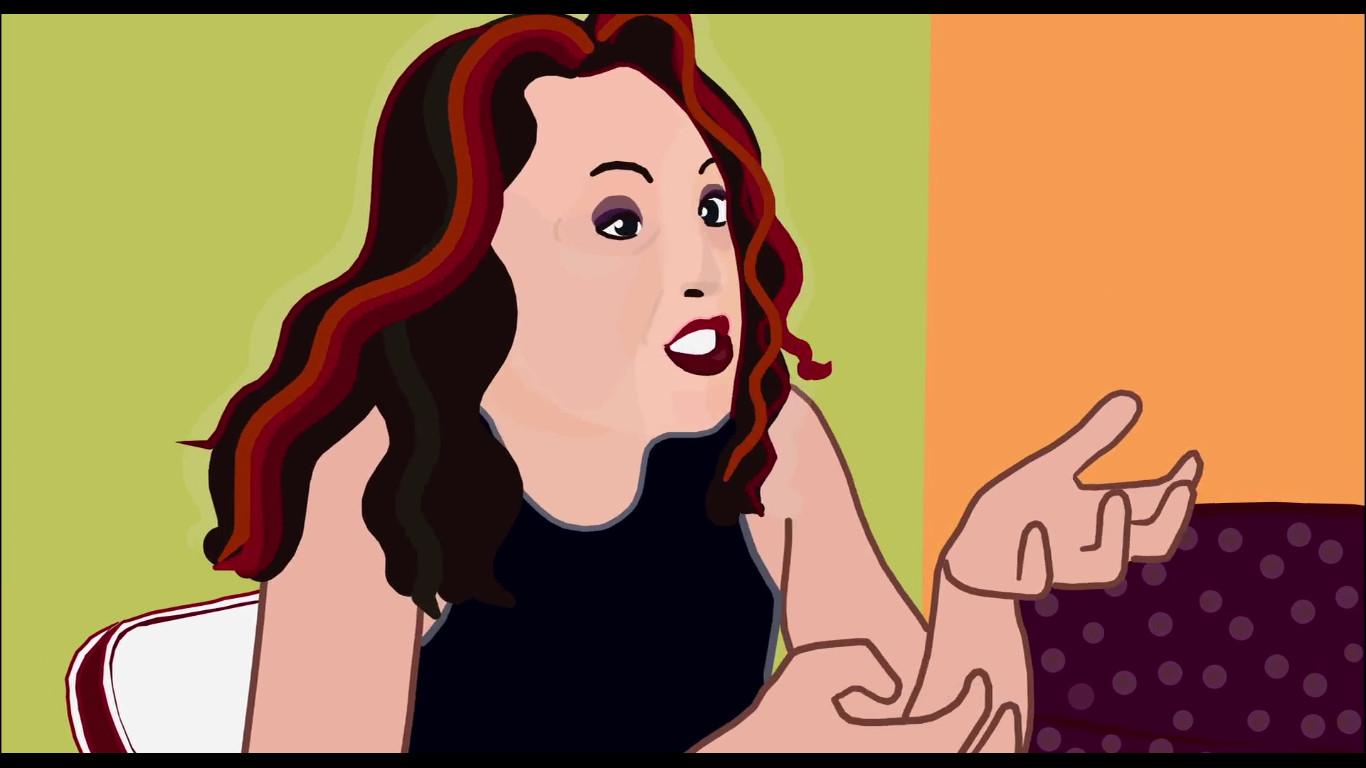
\includegraphics[width=\linewidth]{images/colors}
    \caption{Extrait de \emph{Waking Life (2001)}}
    \label{fig:images_colors}
\end{figure}

Dans \emph{Waking Life (2001)} (figure \ref{fig:images_colors}), l'intégralité
du film est un rêve, presque une excuse pour pouvoir produire un film
entièrement par \textbf{animation rotoscopique}. Cette méthode consiste à
redessiner chaque image filmée pour mêler réalité et fiction, très adapté à
l'exploration du monde onirique.

\subsubsection{Troubles visuels}

\begin{figure}[htpb]
    \centering
    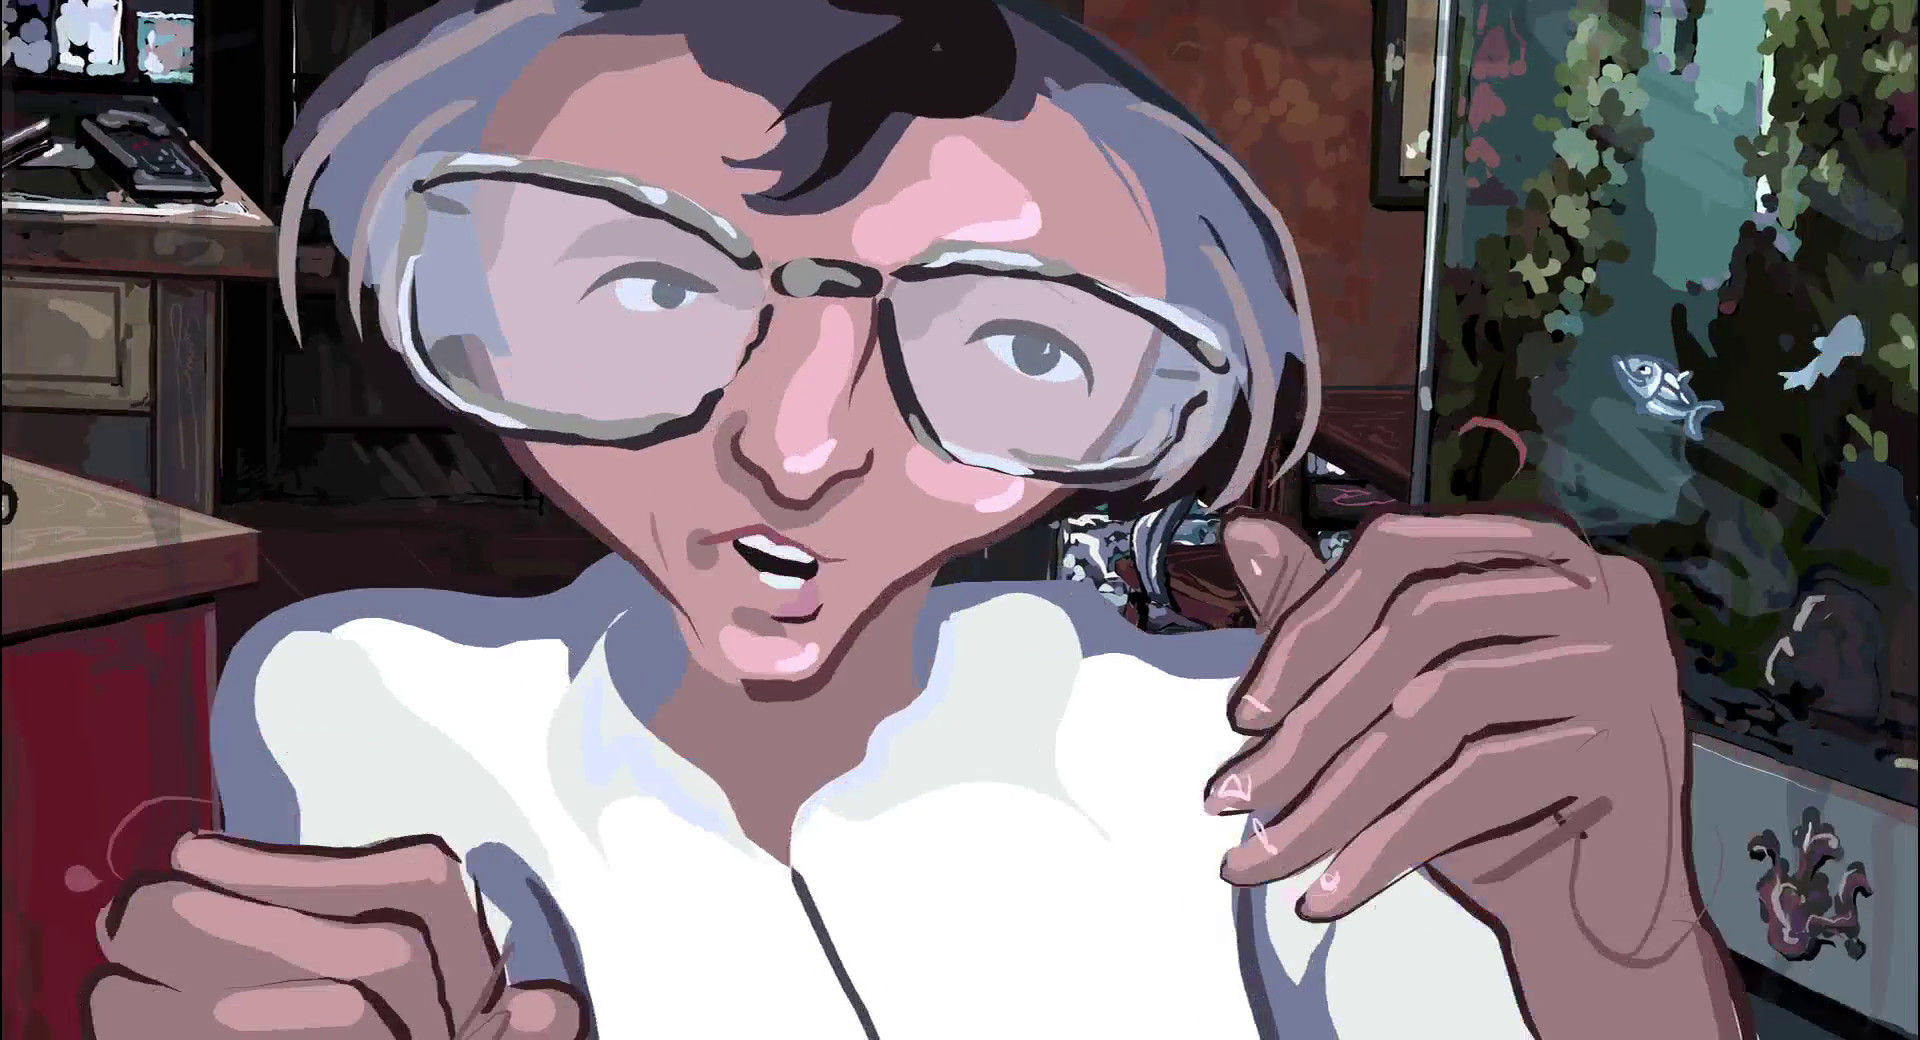
\includegraphics[width=\linewidth]{images/telescopic}
    \caption{Extrait de \emph{Waking Life (2001)}}
    \label{fig:images_telescopic}
\end{figure}

\subsection{Aspect auditif}

\subsection{Symbolisme}

\end{document}
